% Options for packages loaded elsewhere
% Options for packages loaded elsewhere
\PassOptionsToPackage{unicode}{hyperref}
\PassOptionsToPackage{hyphens}{url}
\PassOptionsToPackage{dvipsnames,svgnames,x11names}{xcolor}
%
\documentclass[
  british,
  a4paper,
]{article}
\usepackage{xcolor}
\usepackage{amsmath,amssymb}
\setcounter{secnumdepth}{-\maxdimen} % remove section numbering
\usepackage{iftex}
\ifPDFTeX
  \usepackage[T1]{fontenc}
  \usepackage[utf8]{inputenc}
  \usepackage{textcomp} % provide euro and other symbols
\else % if luatex or xetex
  \usepackage{unicode-math} % this also loads fontspec
  \defaultfontfeatures{Scale=MatchLowercase}
  \defaultfontfeatures[\rmfamily]{Ligatures=TeX,Scale=1}
\fi
\usepackage{lmodern}
\ifPDFTeX\else
  % xetex/luatex font selection
\fi
% Use upquote if available, for straight quotes in verbatim environments
\IfFileExists{upquote.sty}{\usepackage{upquote}}{}
\IfFileExists{microtype.sty}{% use microtype if available
  \usepackage[]{microtype}
  \UseMicrotypeSet[protrusion]{basicmath} % disable protrusion for tt fonts
}{}
\makeatletter
\@ifundefined{KOMAClassName}{% if non-KOMA class
  \IfFileExists{parskip.sty}{%
    \usepackage{parskip}
  }{% else
    \setlength{\parindent}{0pt}
    \setlength{\parskip}{6pt plus 2pt minus 1pt}}
}{% if KOMA class
  \KOMAoptions{parskip=half}}
\makeatother
% Make \paragraph and \subparagraph free-standing
\makeatletter
\ifx\paragraph\undefined\else
  \let\oldparagraph\paragraph
  \renewcommand{\paragraph}{
    \@ifstar
      \xxxParagraphStar
      \xxxParagraphNoStar
  }
  \newcommand{\xxxParagraphStar}[1]{\oldparagraph*{#1}\mbox{}}
  \newcommand{\xxxParagraphNoStar}[1]{\oldparagraph{#1}\mbox{}}
\fi
\ifx\subparagraph\undefined\else
  \let\oldsubparagraph\subparagraph
  \renewcommand{\subparagraph}{
    \@ifstar
      \xxxSubParagraphStar
      \xxxSubParagraphNoStar
  }
  \newcommand{\xxxSubParagraphStar}[1]{\oldsubparagraph*{#1}\mbox{}}
  \newcommand{\xxxSubParagraphNoStar}[1]{\oldsubparagraph{#1}\mbox{}}
\fi
\makeatother


\usepackage{longtable,booktabs,array}
\newcounter{none} % for unnumbered tables
\usepackage{calc} % for calculating minipage widths
% Correct order of tables after \paragraph or \subparagraph
\usepackage{etoolbox}
\makeatletter
\patchcmd\longtable{\par}{\if@noskipsec\mbox{}\fi\par}{}{}
\makeatother
% Allow footnotes in longtable head/foot
\IfFileExists{footnotehyper.sty}{\usepackage{footnotehyper}}{\usepackage{footnote}}
\makesavenoteenv{longtable}
\usepackage{graphicx}
\makeatletter
\newsavebox\pandoc@box
\newcommand*\pandocbounded[1]{% scales image to fit in text height/width
  \sbox\pandoc@box{#1}%
  \Gscale@div\@tempa{\textheight}{\dimexpr\ht\pandoc@box+\dp\pandoc@box\relax}%
  \Gscale@div\@tempb{\linewidth}{\wd\pandoc@box}%
  \ifdim\@tempb\p@<\@tempa\p@\let\@tempa\@tempb\fi% select the smaller of both
  \ifdim\@tempa\p@<\p@\scalebox{\@tempa}{\usebox\pandoc@box}%
  \else\usebox{\pandoc@box}%
  \fi%
}
% Set default figure placement to htbp
\def\fps@figure{htbp}
\makeatother



\ifLuaTeX
\usepackage[bidi=basic,shorthands=off]{babel}
\else
\usepackage[bidi=default,shorthands=off]{babel}
\fi
\ifLuaTeX
  \usepackage{selnolig} % disable illegal ligatures
\fi


\setlength{\emergencystretch}{3em} % prevent overfull lines

\providecommand{\tightlist}{%
  \setlength{\itemsep}{0pt}\setlength{\parskip}{0pt}}



 


\makeatletter
\@ifpackageloaded{tcolorbox}{}{\usepackage[skins,breakable]{tcolorbox}}
\@ifpackageloaded{fontawesome5}{}{\usepackage{fontawesome5}}
\definecolor{quarto-callout-color}{HTML}{909090}
\definecolor{quarto-callout-note-color}{HTML}{0758E5}
\definecolor{quarto-callout-important-color}{HTML}{CC1914}
\definecolor{quarto-callout-warning-color}{HTML}{EB9113}
\definecolor{quarto-callout-tip-color}{HTML}{00A047}
\definecolor{quarto-callout-caution-color}{HTML}{FC5300}
\definecolor{quarto-callout-color-frame}{HTML}{acacac}
\definecolor{quarto-callout-note-color-frame}{HTML}{4582ec}
\definecolor{quarto-callout-important-color-frame}{HTML}{d9534f}
\definecolor{quarto-callout-warning-color-frame}{HTML}{f0ad4e}
\definecolor{quarto-callout-tip-color-frame}{HTML}{02b875}
\definecolor{quarto-callout-caution-color-frame}{HTML}{fd7e14}
\makeatother
\makeatletter
\@ifpackageloaded{caption}{}{\usepackage{caption}}
\AtBeginDocument{%
\ifdefined\contentsname
  \renewcommand*\contentsname{Table of contents}
\else
  \newcommand\contentsname{Table of contents}
\fi
\ifdefined\listfigurename
  \renewcommand*\listfigurename{List of Figures}
\else
  \newcommand\listfigurename{List of Figures}
\fi
\ifdefined\listtablename
  \renewcommand*\listtablename{List of Tables}
\else
  \newcommand\listtablename{List of Tables}
\fi
\ifdefined\figurename
  \renewcommand*\figurename{Figure}
\else
  \newcommand\figurename{Figure}
\fi
\ifdefined\tablename
  \renewcommand*\tablename{Table}
\else
  \newcommand\tablename{Table}
\fi
}
\@ifpackageloaded{float}{}{\usepackage{float}}
\floatstyle{ruled}
\@ifundefined{c@chapter}{\newfloat{codelisting}{h}{lop}}{\newfloat{codelisting}{h}{lop}[chapter]}
\floatname{codelisting}{Listing}
\newcommand*\listoflistings{\listof{codelisting}{List of Listings}}
\makeatother
\makeatletter
\makeatother
\makeatletter
\@ifpackageloaded{caption}{}{\usepackage{caption}}
\@ifpackageloaded{subcaption}{}{\usepackage{subcaption}}
\makeatother
\usepackage{bookmark}
\IfFileExists{xurl.sty}{\usepackage{xurl}}{} % add URL line breaks if available
\urlstyle{same}
% fallback for those not using the hyperref driver hyperxmp:
\makeatletter
\@ifundefined{xmpquote}{\newcommand{\xmpquote}[1]{#1}}{}
\makeatother
\hypersetup{
  pdftitle={An emerging-market briefing in days{,} from a model that knows when not to trade},
  pdfauthor={Carlos Galindo},
  pdflang={en-GB},
  colorlinks=true,
  linkcolor={blue},
  filecolor={Maroon},
  citecolor={Blue},
  urlcolor={Blue},
  pdfcreator={LaTeX via pandoc}}


\title{An emerging-market briefing in days, from a model that knows when
not to trade}
\usepackage{etoolbox}
\makeatletter
\providecommand{\subtitle}[1]{% add subtitle to \maketitle
  \apptocmd{\@title}{\par {\large #1 \par}}{}{}
}
\makeatother
\subtitle{The projection model applied at short notice to Egypt, where
public debt is partly in foreign currency, and then broadened to labour
markets, supply capacity, fiscal policy and public debt management}
\author{Carlos Galindo}
\date{}
\begin{document}
\maketitle


\begin{tcolorbox}[enhanced jigsaw, arc=.35mm, bottomrule=.15mm, breakable, colback=white, colframe=quarto-callout-note-color-frame, left=2mm, leftrule=.75mm, opacityback=0, rightrule=.15mm, toprule=.15mm]

\vspace{-3mm}\textbf{At a glance}\vspace{3mm}

\begin{itemize}
\tightlist
\item
  \textbf{Question.} Can a framework built and tested on advanced
  economies brief an emerging market with foreign-currency debt at short
  notice, without cutting corners on the evidence?
\item
  \textbf{Approach.} The same calibrated projection model and the same
  evidence standard, applied to Egypt within days. The evidence chose
  the regime, and the briefing ran from the country's macroeconomic
  position to scenarios, a watch-list and, on request, trade ideas.
\item
  \textbf{Finding.} The framework placed Egypt on the foreign-currency
  path and brought out the two-sided effect of high real interest rates:
  they support the currency and pull inflation down, and they raise the
  public interest bill. Both effects last only while foreign inflows
  continue.
\item
  \textbf{Why it matters.} Speed and rigour usually trade off. Here the
  speed comes from the framework itself, and the rigour comes from a
  standard that marks every gap in the evidence and declines to
  recommend anything the evidence cannot carry.
\end{itemize}

\end{tcolorbox}

\subsection{The question}\label{the-question}

A country briefing written at short notice tends to fail in one of two
ways. It is either thin, because there was no time to build a view, or
confident beyond its evidence, because the gaps were filled with
plausible numbers. Emerging markets make both failures more likely. The
data are released with longer lags, the official and market sources
disagree more often, and the price that can break is not always the one
an advanced-economy reader expects to watch.

The framework had been built to read advanced and emerging economies
with one model, letting the currency in which public and bank debt is
owed decide where a funding shock lands. Its first application covered
five advanced economies, all of which borrow in their own currency. The
open test was the other side of the fork: an economy whose government
owes a large part of its debt in foreign currency, relies on foreign
holders of its local bills, and sits close to the end of an IMF
programme. Egypt fits that description, and the author last covered it
in co-authored sell-side research in 2017. The question was whether the
framework could carry a full briefing on it within days.

\subsection{Approach}\label{approach}

\textbf{The evidence chooses the regime.} The model does not assume that
a country is an emerging market. It tests the debt structure first, in a
fixed order, and the first test the evidence passes decides which block
of the model applies. For Egypt the evidence pointed to the
foreign-currency path: material external public debt, a large share of
local bills held by non-residents, and repayments falling due within the
year. On that path the objects to watch are reserve cover, external
repayments and the willingness of foreign investors to keep rolling
their bills, rather than the long-end auction that dominates an advanced
economy's reading.

\textbf{One standard for every figure.} Every number in the briefing
carries a grade: established from a named official source, inferred with
its method stated, or not identified. Official producers come first: the
central bank, the statistics office and the finance ministry, with
international institutions and rating agencies as confirmation. Where
two sources disagreed, both were set side by side and the one used was
named. Where a series was not published for Egypt, the briefing said so
and set no trigger on it.

\textbf{Trade ideas are optional and conditional.} The same framework
that writes the briefing can, on request, turn it into market positions.
Each position must be tied to a mechanism in the briefing, carry an exit
condition stated as an observable event, and be sized from a stated risk
budget. Where the evidence for any of these is missing, the output is
not a weaker trade but no trade, with the missing inputs named.

\textbf{One evidence base, several readers.} From the same graded
evidence the framework produced a desk-style briefing, a short research
abstract and plain-language explanations for readers without an
economics background. The figures and their grades are identical across
all three; only the register changes.

\subsection{What the work shows}\label{what-the-work-shows}

\textbf{The regime fork works on the other side.} The model that read
five advanced economies on the local-currency path read Egypt on the
foreign-currency path, using the same equations. The difference sits
where the economics puts it: in which stock can break, and therefore in
which prices and releases deserve attention.

\textbf{High real rates cut both ways.} The central finding of the
briefing is a mechanism, not a forecast. A policy rate well above
inflation draws foreign money into local bills, supports the currency,
and keeps import prices, and so inflation, on a downward path. The same
rate raises the share of government revenue spent on interest, which
strains the fiscal credibility on which the inflows depend. While
inflows continue, the first effect dominates. If they stop, the sign
flips: the currency weakens, pass-through raises prices, and policy is
pushed to tighten into a heavier interest bill. The first figure shows
the shape of that fork on simulated data.

\begin{figure}

\centering{

\pandocbounded{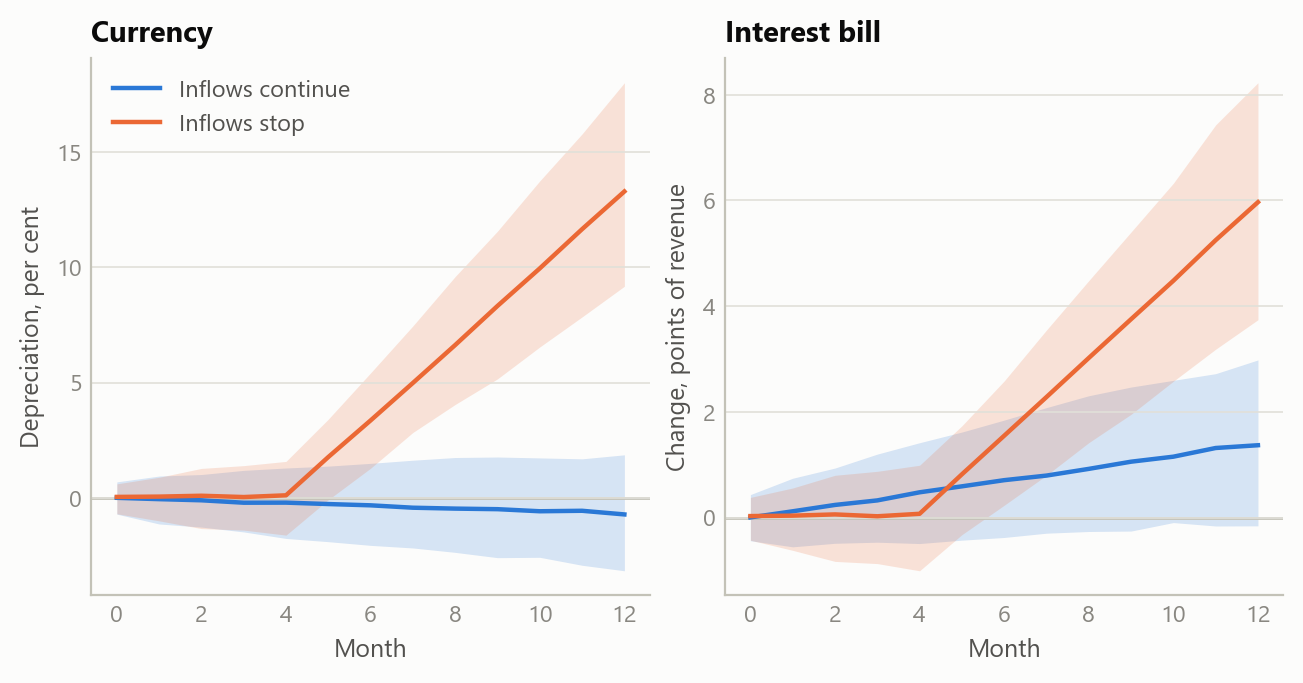
\includegraphics[keepaspectratio]{index_files/figure-latex/fig-fork-output-1.png}}

}

\caption{\label{fig-fork}One high-real-rate regime under two paths for
foreign inflows: median and 90\% band of the currency and of the public
interest bill over twelve months (simulated data).}

\end{figure}%

\textbf{Scenarios are tied to a test.} The briefing set out three
scenarios, a base case, an upside and a tail, each starting from a
different event and each carrying a falsifier: a named release and the
level at which it would show the scenario to be wrong. The end of the
IMF programme stood out as the clearest dated test of whether the
inflows, and so the favourable side of the fork, would hold.

\textbf{The gaps are part of the output.} A briefing that marks what it
could not find is more useful than one that hides it, because the gap
tells the reader where the risk of being surprised is largest. The
second figure shows, on simulated data, the kind of evidence ledger the
standard produces: the share of figures in each part of a briefing that
are established, inferred or not identified. The later, more judgemental
parts carry more inference by design, and trade ideas are issued only
where their evidence conditions are met.

\begin{figure}

\centering{

\pandocbounded{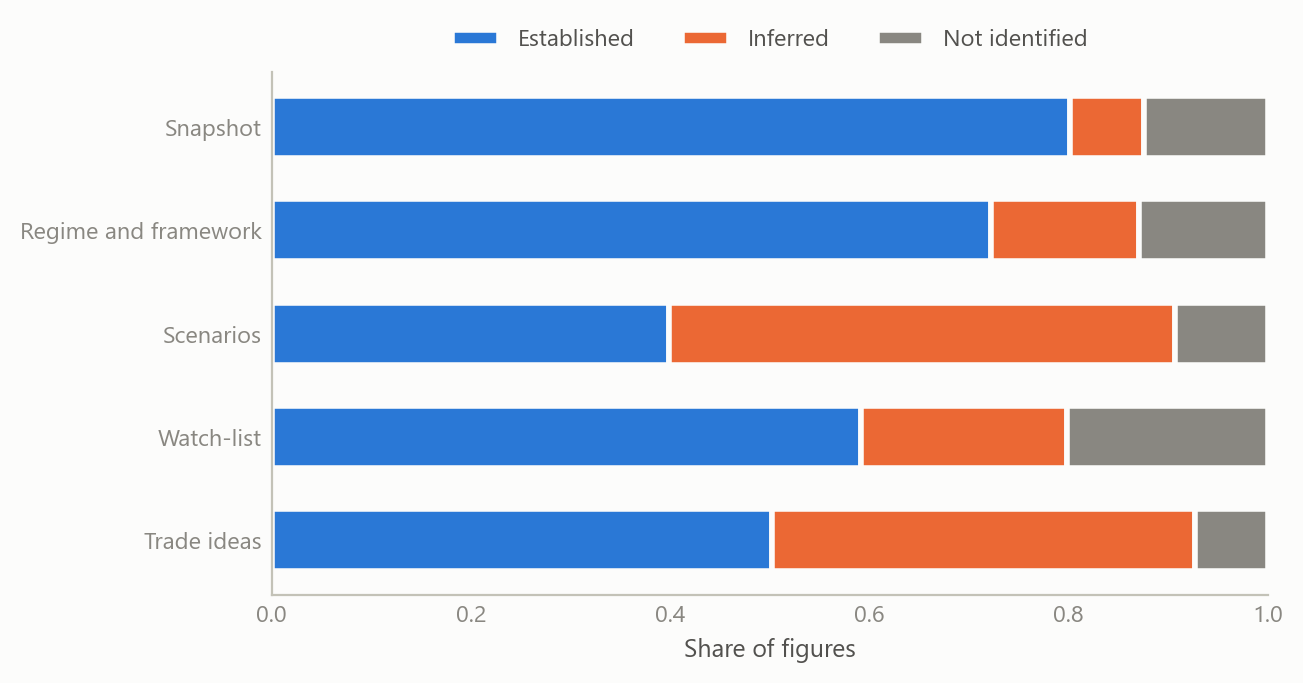
\includegraphics[keepaspectratio]{index_files/figure-latex/fig-ledger-output-1.png}}

}

\caption{\label{fig-ledger}Evidence ledger of a country briefing: share
of figures established, inferred or not identified, by part of the
briefing (simulated data).}

\end{figure}%

\textbf{The framework grew from the exercise.} Applying it to an
emerging market under time pressure showed where it was thin, and the
specification was then broadened to cover labour markets, supply
capacity, aggregate demand, fiscal policy and public debt management in
one integrated reading. Fiscal decisions are now traced step by step,
from announcement and legal status through financing, demand, wages and
prices, to the central bank, the bond curve and the currency, and back
to the budget, with the chain stopping at the first link the evidence
cannot support.

\textbf{Follow-up questions run on the same standard.} The framework
then answered three narrower questions on the same country: whether it
can keep servicing its foreign debt, how the politics of official
financing enter that answer as its IMF programme ends, and whether a
disruption to imported food changes it. Each answer was traced back into
the same loop between real rates, foreign inflows and the interest bill,
and each stopped where the evidence stopped. The foreign debt is
manageable on its present path only while maturing obligations keep
being rolled over and the currency holds. Politics matters through the
official inflows that keep that rollover going and through the anchor
that the programme's end removes. The food shock tightens the loop at
the margin without becoming the trigger.

\subsection{Insights}\label{insights}

\begin{enumerate}
\def\labelenumi{\arabic{enumi}.}
\tightlist
\item
  \textbf{Speed comes from the framework, not from shortcuts.} A model
  that already knows which questions decide a country's risk turns days
  of preparation into a briefing that can be read and challenged line by
  line.
\item
  \textbf{The same instrument can support and threaten.} A high real
  interest rate can buy disinflation and a stable currency while raising
  the fiscal cost that sustains them. Which effect dominates depends on
  a flow, foreign inflows, that can stop.
\item
  \textbf{Knowing when not to trade is a feature.} A recommendation that
  cannot name its exit, its size and its evidence is withheld, with the
  missing inputs listed. That discipline is what makes the
  recommendations that are issued worth reading.
\item
  \textbf{A marked gap is information.} The places where the evidence is
  not identified are where the next release can surprise most, and the
  briefing says so instead of filling them.
\item
  \textbf{One evidence base can serve every reader.} Graded evidence can
  be written up for a trading desk, a policy reader or a non-specialist
  without the numbers changing between versions.
\item
  \textbf{A shock that tightens is not a shock that breaks.} A dearer
  import bill can keep interest rates higher for longer and the public
  interest bill heavier, but the path flips only if financing stops.
  Keeping the two apart stops a briefing from reading every new headline
  as a crisis.
\end{enumerate}

\subsection{Scope and next steps}\label{scope-and-next-steps}

The framework reads an emerging market with foreign-currency debt and an
advanced economy with local-currency debt on one calibrated model, and
can deliver a graded country briefing at short notice, with market
positions available on request and withheld where the evidence is short.

The natural extensions are three. First, the broadened specification,
with its labour, supply and fiscal blocks, applied across the Middle
East and North Africa and to hybrid cases where both debt blocks run at
once. Second, the briefing tracked through time, so that each scenario's
falsifier is checked against the release that tests it. Third, a policy
version of the output, in which the fiscal transmission map is read for
its implications for official lending, programme design and spillovers
to the UK.

The full specification, the country briefing and its plain-language
versions can be discussed on request.

\subsection{About the evidence}\label{about-the-evidence}

The work was done in October 2026. It rests on the written model
specification, a full country briefing on Egypt with its scenarios,
watch-list and trade ideas, a short research abstract, a plain-language
explanation for non-specialists, the broadened specification written
after the exercise, and three follow-up assessments (external-debt
sustainability, the politics of official financing, and a supply shock
to imported food), two of them with plain-language versions. The
coefficients are calibration priors, not estimates. The market and
fiscal figures behind the briefing are not reproduced here. The two
figures are simulated, built to share the structure of the analysis (a
two-path fork for foreign inflows, an evidence ledger by part of the
briefing); neither shows a real estimate.

Figures and tables marked \emph{simulated} are generated from simulated
data built to share the structure of the analysis (its variables,
horizons and frequencies). They show how each method works and what its
output looks like. Results stated in the text, and figures that give a
source, are the project's own. Methods are described at the level of a
methods section. Code and data pipelines are not reproduced here.




\end{document}
